% =============================================================================
% ch04_slam.tex — Chapter 4: SLAM Algorithms | Biomimetic Navigator
% =============================================================================

\selectlanguage{hebrew}
\section{אלגוריתמי \en{SLAM} ביומימטיים}
\label{sec:slam}

\subsection{מבוא ל-\en{SLAM} הסתברותי}
בעיית ה-\en{SLAM} (\en{Simultaneous Localization and Mapping}) מוגדרת כניסיון לאמוד בו-זמנית את מצב הרחפן $\mathbf{x}_t$ ואת מפת הסביבה $\mathcal{M}$ בהינתן סדרת תצפיות $\mathbf{z}_{1:t}$ ופקודות בקרה $\mathbf{u}_{1:t}$. אנו משתמשים בגישות בייזיאניות כדי לנהל את אי-הוודאות המובנית בתהליך זה. \cite{Thrun2005ProbRobotics}

% ── NEW: Acoustic Fovea & AF-AFC ────────────────────────────────────────────
\subsection{פוביית האקוסטיקה ומפצה הדופלר האדפטיבי}
\label{subsec:acoustic_fovea}

\subsubsection{הבסיס הביולוגי: ה\en{Acoustic Fovea}}
\label{subsubsec:fovea_bio}

עטלפי-פרסה (\textit{Rhinolophus ferrumequinum}) מפגינים תופעה ביולוגית
יוצאת-דופן הידועה כ\textbf{פיצוי תזוזת דופלר}
(\en{Doppler Shift Compensation — DSC}) \cite{Schnitzler1968DSC}.
קליפת-השבלול שלהם מכילה אזור יֶתֶר-ייצוג עצבי צר-תדר
סביב תדר ה-\en{CF} של הקריאה ($f_0 \approx 83\,\text{kHz}$)
המכסה כ-30\% מהממברנה הבזאלית, הנקרא ה\textbf{\en{acoustic fovea}}.

בזמן טיסה, תנועת העטלף כלפי מטרה מוסיפה תזוזת-דופלר $\Delta f_D > 0$
לתדר ההד (\en{echo}), וכתוצאה מכך ההד מתרחק מאזור הפוביה.
במנגנון רפלקסיבי עם השהייה $\lesssim 20\,\text{ms}$,
גזע-המוח \textbf{מוריד} את תדר הפליטה ב-$\Delta f_D$
כדי שההד יחזור ל-$f_0$. \cite{Schuller1974DSC}
מנגנון זה מקנה לעטלף רזולוציה-מהירות (\en{velocity resolution})
הגבוהה ממערכות \en{FMCW} מלאכותיות בסדר-גודל.

\subsubsection{מימוש מלאכותי: בקר AF-AFC}
\label{subsubsec:afafc}

מנגנון ה\en{DSC} מתורגם למערכת הרחפן כ\textbf{בקר תדר-פליטה אדפטיבי}
(\en{Adaptive Frequency — Acoustic Fovea Controller, AF-AFC}).
עבור מערך של $K$ קרניים אקוסטיות, הקרן ה-$k$ פולטה בתדר $f_{e,k}(t)$
המחושב בזמן-אמת מהאמדן האחורי של ה-\en{EKF}.

המרכיב הרדיאלי של מהירות הרחפן לכיוון קרן $k$:
\begin{equation}
    \hat{v}_{r,k}(t)
    = \hat{\mathbf{v}}_{\mathrm{ego}}(t)\cdot\hat{\mathbf{n}}_k,
    \qquad
    \hat{\mathbf{n}}_k = \begin{pmatrix}
        \cos\phi_k\cos\theta_k\\
        \cos\phi_k\sin\theta_k\\
        \sin\phi_k
    \end{pmatrix}
    \label{eq:radial_vel}
\end{equation}
כאשר $(\theta_k, \phi_k)$ הם זווית-האמוצ'יה (\en{azimuth})
וזווית-ההגבהה (\en{elevation}) של קרן $k$,
ו-$\hat{\mathbf{v}}_{\mathrm{ego}}(t)$ מחולץ מוקטור-המצב האחורי
$\hat{\mathbf{x}}_{t|t}$ של ה-\en{EKF} (משוואה~\ref{eq:ekf_update}).

שגיאת הפוביה (\en{foveal error}), כלומר סטיית תדר ההד מ-$f_0$,
מוגדרת כ:
\begin{equation}
    \varepsilon_k(t) = f_{\mathrm{echo},k}(t) - f_0
    \label{eq:foveal_error}
\end{equation}
ומחושבת בזמן-אמת על-ידי זיהוי-שיא (\en{peak detection})
בפלט מסנן-ההתאמה $y_k(\tau)$ (משוואה~\ref{eq:range_resolution}).

\textbf{בקר ה-AF-AFC} משלב פיצוי-קדימה (\en{feedforward})
המבוסס על אמדן-ה\en{EKF} עם תיקון-משוב (\en{feedback}) לטיפול
בשגיאות מודל:
\begin{equation}
    \boxed{
    f_{e,k}(t)
    = f_0\!\left(1 - \frac{2\,\hat{v}_{r,k}(t)}{c}\right)
    + \underbrace{K_p\,\varepsilon_k(t)
    + K_i\!\int_0^t \varepsilon_k(\tau)\,d\tau}_{\text{תיקון-משוב PI}}
    }
    \label{eq:afafc}
\end{equation}

האיבר הראשון ($f_0\,(1-2\hat{v}_r/c)$) הוא תרגום ישיר של מנגנון
ה\en{DSC} הביולוגי; מרכיב ה-\en{PI} ($K_p, K_i$) מקביל לפלסטיות
הסינפטית (\en{synaptic plasticity}) ב\en{inferior colliculus}
המתגמשת לאורך זמן. ערכי ברירת-מחדל: $K_p = 0.8$, $K_i = 0.05\,\text{s}^{-1}$.

\paragraph{השפעה על רזולוציית הטווח.}
מבלעדי פיצוי, תזוזת-דופלר גורמת לסטייה (\en{smearing})
של שיא מסנן-ההתאמה ברזולוציה:
\begin{equation}
    \Delta r_{\mathrm{uncomp}}
    = \frac{c}{2B}\cdot\frac{1}{1 - 2v_{r,k}/c}
    \approx \frac{c}{2B}\!\left(1 + \frac{2v_{r,k}}{c}\right)
    \label{eq:range_smear}
\end{equation}
לאחר פיצוי ה\en{AF-AFC}, הסטייה מצטמצמת ל:
\begin{equation}
    \Delta r_{\mathrm{comp}}
    = \frac{c}{2B}\cdot\frac{\left|\varepsilon_k(t)\right|}{f_0}
    \xrightarrow{\varepsilon_k \to 0}\ \frac{c}{2B} = \Delta r_{\mathrm{ideal}}
    \label{eq:range_comp}
\end{equation}
כלומר, בגבול $\varepsilon_k \to 0$ הרזולוציה חוזרת לגבול-הרייקלי
(\en{Rayleigh limit}) $\Delta r = c/2B$, ללא תלות במהירות הרחפן,
בדיוק כפי שה\en{acoustic fovea} מספקת לעטלף רזולוציה קבועה
על-פני טווח מהירויות $0$–$9\,\text{m/s}$. \cite{Simmons1979BatSonar}
% ────────────────────────────────────────────────────────────────────────────

\subsection{מסנן קלמן המורחב (\en{EKF-SLAM})}
ה-\en{EKF-SLAM} הוא אחד האלגוריתמים הבסיסיים והנפוצים ביותר. הוא מניח כי מצב המערכת והתצפיות מתפלגים גאוסיאנית. התהליך מחולק לשני שלבים:
\begin{enumerate}
    \item \textbf{שלב הניבוי (\en{Predict}):} עדכון המצב על סמך מודל התנועה.
    \item \textbf{שלב העדכון (\en{Update}):} תיקון המצב על סמך התצפיות מהחיישנים. משוואת עדכון המצב היא:
\begin{equation}
    \hat{\mathbf{x}}_{t|t} = \hat{\mathbf{x}}_{t|t-1} + \mathbf{K}_t (\mathbf{z}_t - h(\hat{\mathbf{x}}_{t|t-1}))
    \label{eq:ekf_update}
\end{equation}
\end{enumerate}

גידול וצמצום אי-הוודאות (המיוצגת על ידי מטריצת הקווריאנס $P$) מוצגים באיור \ref{fig:ekf_covariance}:

\begin{figure}[H]
    \centering
    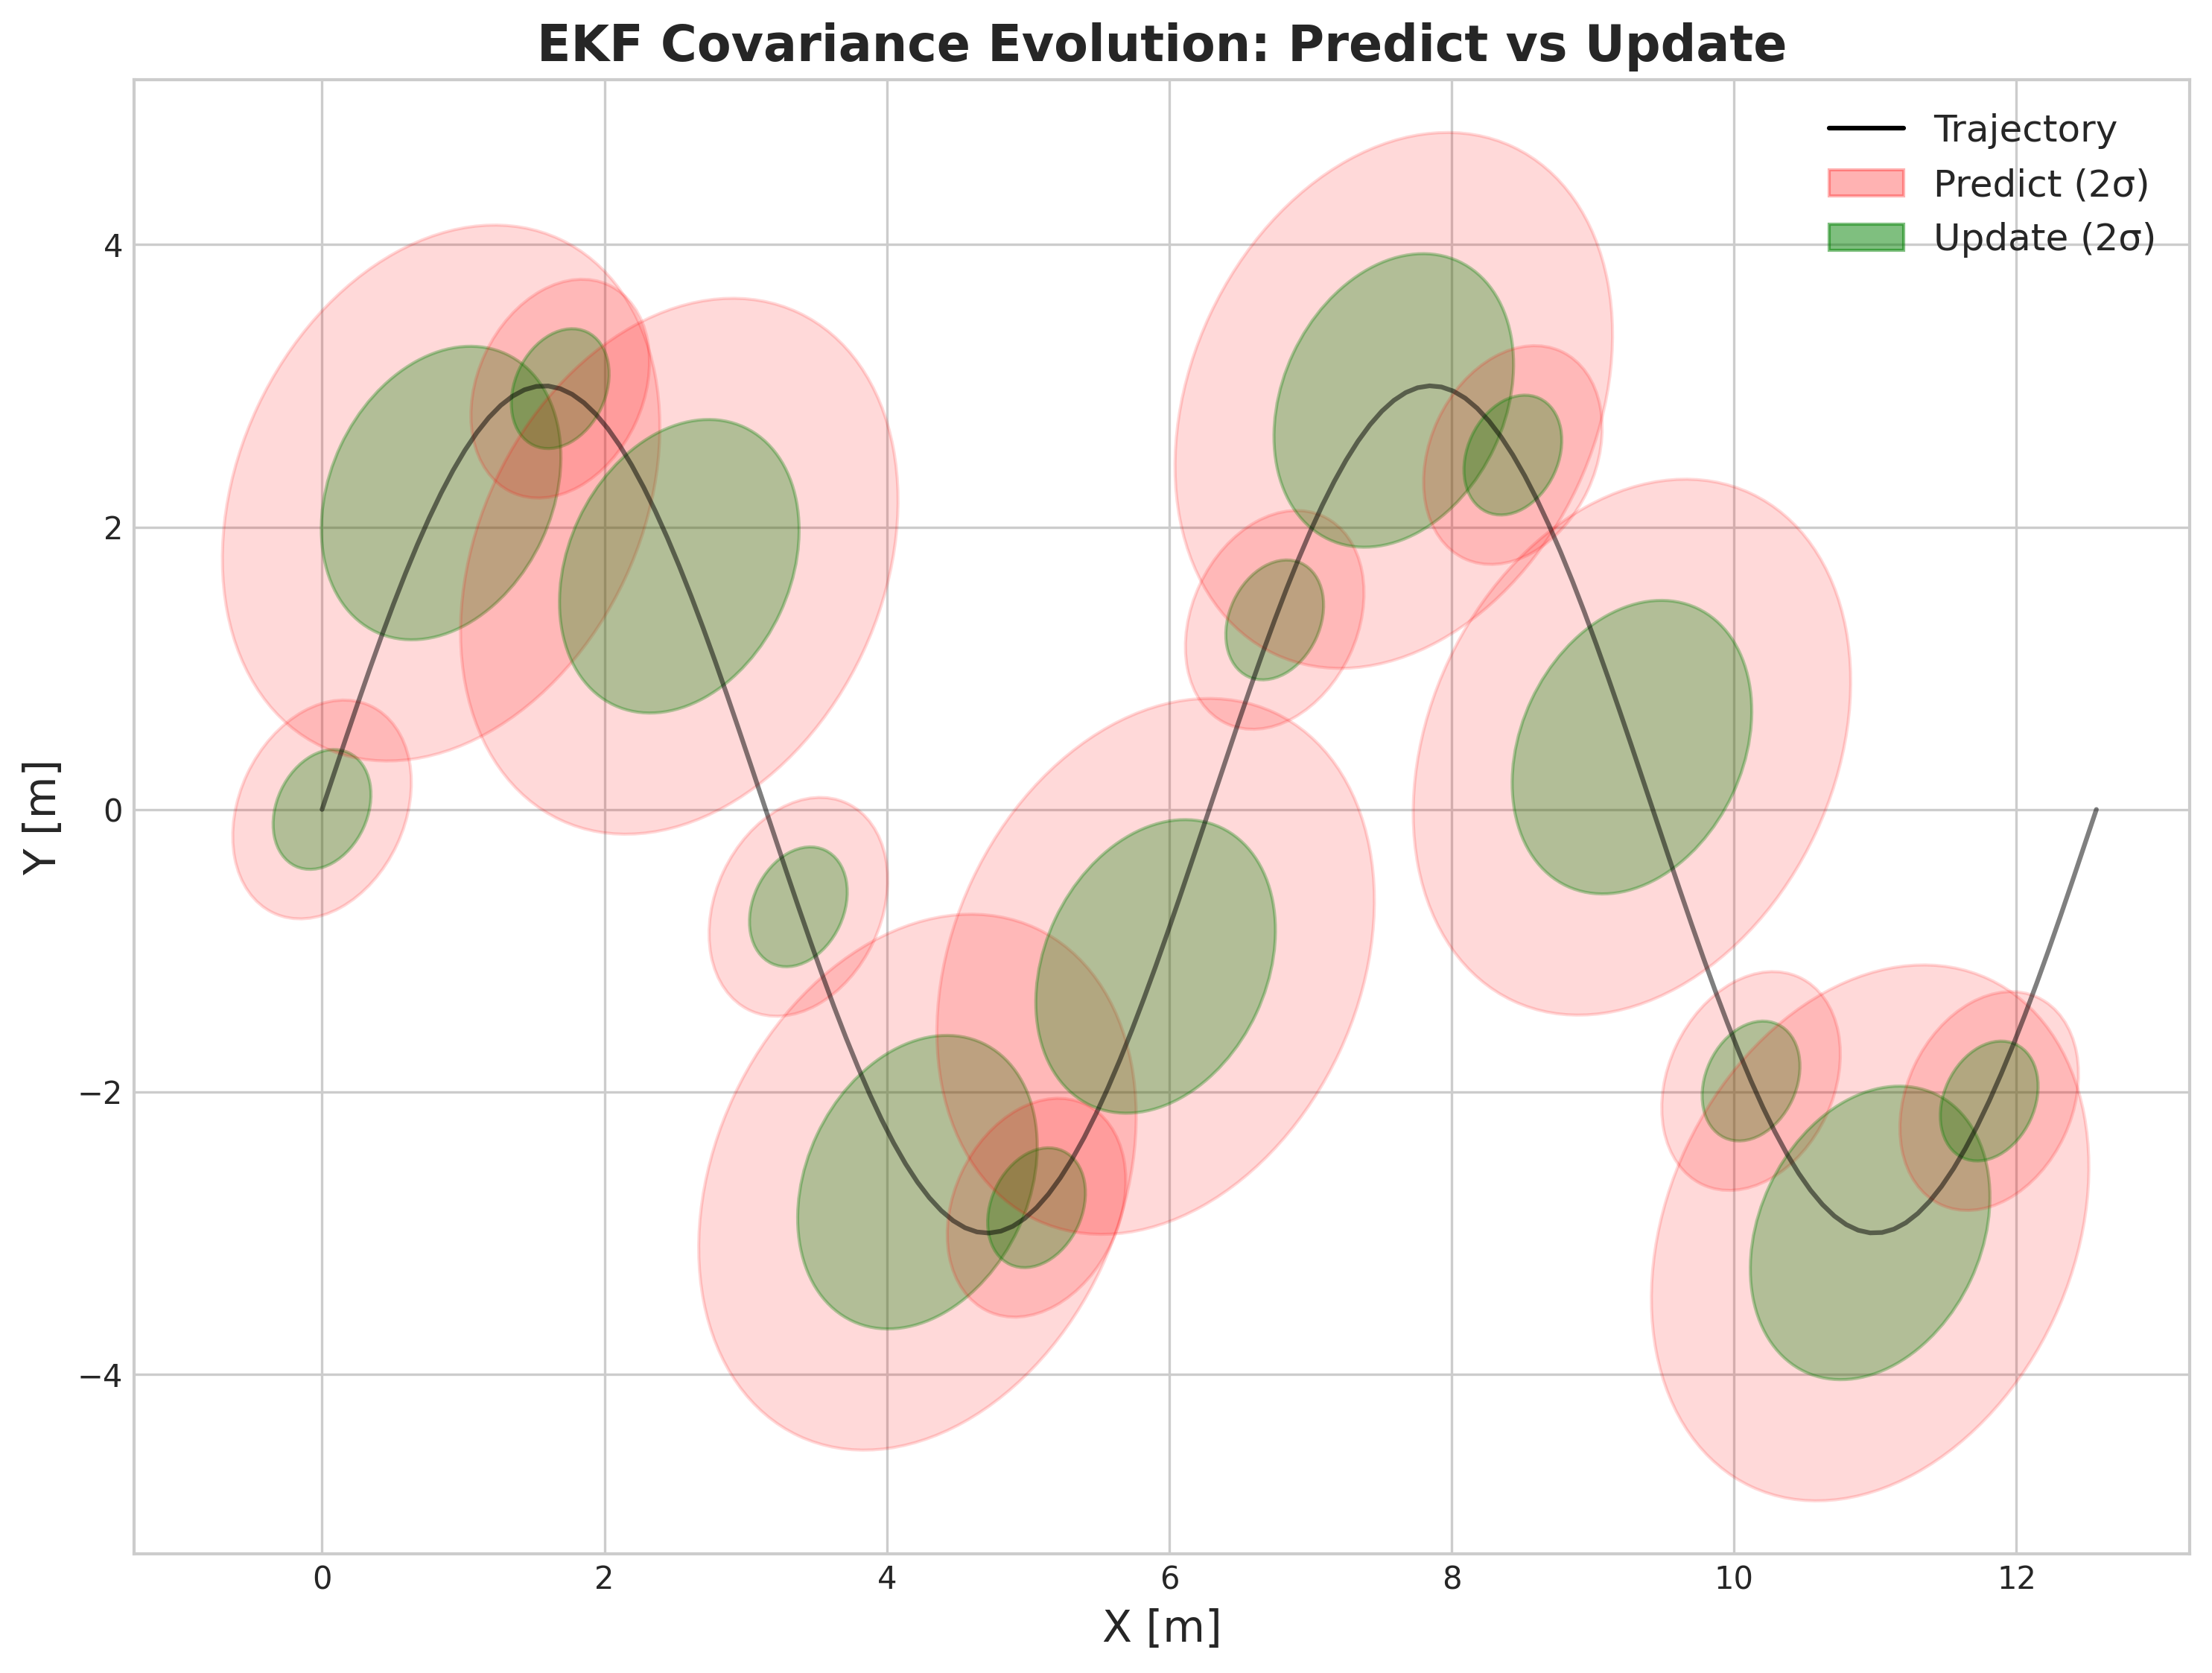
\includegraphics[width=0.8\columnwidth]{figures/fig_ekf_covariance.png}
    \caption{אליפסות קווריאנס של \en{EKF}. ניתן לראות כיצד אי-הוודאות גדלה במהלך התנועה ומצטמצמת בעת קבלת תצפית מהחיישנים.}
    \label{fig:ekf_covariance}
\end{figure}

\subsection{אופטימיזציית גרף (\en{Graph-SLAM})}
בעוד ש-\en{EKF} שומר רק על המצב הנוכחי, \en{Graph-SLAM} שומר על כל היסטוריית המצבים כצמתים בגרף. הקשרים בין הצמתים (מגבלות, \en{constraints}) מיוצגים על ידי קשתות. מטרת האלגוריתם היא למצוא את מערך המצבים $\mathbf{x}^*$ שממזער את שגיאת הריבועים המינימלית:
\begin{equation}
    \mathbf{x}^* = \arg\min_{\mathbf{x}} \sum_{i} e_i(\mathbf{x})^\top \Omega_i e_i(\mathbf{x})
    \label{eq:graph_opt}
\end{equation}
כאשר $e_i$ היא פונקציית השגיאה ו-$\Omega_i$ היא מטריצת האינפורמציה (ההופכית לקווריאנס). \cite{Grisetti2010g2o}

\subsection{\en{ORB-SLAM3} כנקודת ייחוס}
כנקודת השוואה סטנדרטית, אנו משתמשים ב-\en{ORB-SLAM3}, המשלב תכונות חזותיות (\en{visual features}) עם נתוני \en{IMU}. זהו אלגוריתם חזק מאוד אך הוא סובל מקשיים בסביבות דלות בטקסטורה או בחשיכה, שם הסונאר הביומימטי שלנו מצטיין. \cite{MurArtal2015ORB}

\subsection{השוואת ביצועי אלגוריתמים}
בטבלה \ref{tab:slam_comparison} אנו משווים בין הגישות השונות בהיבטי דיוק וסיבוכיות חישובית.

\begin{table}[H]
\centering
\begin{tabular}{lccc}
\toprule
אלגוריתם & דיוק לוקליזציה & סיבוכיות & חסינות לרעש \\
\midrule
\en{EKF-SLAM} & בינוני & $O(N^2)$ & בינונית \\
\en{Graph-SLAM} & גבוה & $O(N)$ (דליל) & גבוהה \\
\en{ORB-SLAM3} & גבוה מאוד & גבוהה & נמוכה (בחושך) \\
\bottomrule
\end{tabular}
\caption{השוואת אלגוריתמי \en{SLAM} נבחרים.}
\label{tab:slam_comparison}
\end{table}
